\section{Solving Burger's equation using Fourier Galerkin}

This section explores the Fourier Galerkin method for solving the Burgers' equation:
\begin{equation}
	\frac{\partial u(x, t)}{\partial t} + u(x, t) \frac{\partial u(x, t)}{\partial x} = \nu \frac{\partial^2 u(x, t)}{\partial x^2}
\end{equation}
with the same parameters ($c = 4.0$ and $\nu = 0.1$) and periodic boundary conditions on $x \in [0, 2\pi]$.

The Fourier Galerkin method expands the solution in terms of Fourier modes:
\begin{equation}
	u(x, t) = \sum_{n=-N/2}^{N/2} \hat{u}_n(t)e^{inx}
\end{equation}
where $\hat{u}_n(t)$ are the time-dependent Fourier coefficients. Unlike the Collocation method which satisfies the PDE at specific grid points, the Galerkin method requires the residual to be orthogonal to each basis function, leading to a system of ODEs for the Fourier coefficients.

The key algorithmic difference lies in the treatment of nonlinear terms: the Galerkin method transforms between physical and spectral space, computing the nonlinear term $u\frac{\partial u}{\partial x}$ in physical space before transforming back to spectral space for time integration. This approach requires careful dealiasing to prevent spectral aliasing errors, which proved to be a critical implementation challenge.

For time integration, we used the same 4th-order Runge-Kutta scheme as in Part 2, but with a modified time step restriction:
\begin{equation}
	\Delta t \leq \text{CFL} \times \left[ \max_{x_j} \left(|u(x_j)| k_{max} + \nu (k_{max})^2  \right)\right]^{-1}
\end{equation}
where $k_{max} = N/2$ is the maximum wavenumber in the spectral representation.

\subsection{Dealiasing Implementation}

The implementation of the Fourier Galerkin method required careful management of aliasing errors arising from the nonlinear term $u\frac{\partial u}{\partial x}$. When computed in physical space, this product generates frequencies up to $2k_{max}$ that exceed the spectral resolution, causing aliasing when transformed back to spectral space.

\subsubsection{Dealiasing Strategy}
To prevent aliasing instabilities, the standard 2/3 dealiasing rule was implemented for all grid sizes:

\begin{equation}
	k_{cutoff} = \frac{2k_{max}}{3} = \frac{N}{3}
\end{equation}

The dealiasing algorithm operates as follows:
\begin{enumerate}
	\item Compute nonlinear term $u\frac{\partial u}{\partial x}$ in physical space
	\item Transform to spectral space using FFT
	\item Apply dealiasing filter: $\hat{f}_k = 0$ for $|k| > k_{cutoff}$
	\item Use filtered coefficients in time integration
\end{enumerate}

\subsubsection{Impact on Results}
The dealiasing implementation was essential for numerical stability:

\begin{itemize}
	\item \textbf{Stability Enhancement}: Enabled stable computation up to $N = 256$, preventing the exponential error growth characteristic of aliasing instabilities
	\item \textbf{Convergence Improvement}: Transformed initially chaotic convergence behavior into meaningful spectral convergence rates for most grid sizes
	\item \textbf{Residual Challenges}: Despite dealiasing, certain grid sizes ($N = 64, 256$) exhibited suboptimal convergence, indicating potential resonance effects or insufficient dealiasing for these specific cases
\end{itemize}

This demonstrates that while the 2/3 rule provides a robust foundation for aliasing control in spectral methods, problem-specific tuning may be necessary for optimal performance across all grid resolutions.

\subsection{Determining Maximum CFL Values}

\subsubsection{Methodology}
The maximum stable CFL values for the Fourier Galerkin method were determined using the same incremental testing approach as in Section 2, but adapted for the spectral formulation. The algorithm proceeds as follows:

\begin{enumerate}
	\item \textbf{Incremental Testing}: For each grid size $N$, CFL values are tested incrementally starting from 3.0 with steps of 0.05, reflecting the generally higher stability limits of Galerkin methods compared to collocation.
	\item \textbf{Stability Criterion}: A solution is considered stable if:
	      \begin{itemize}
		      \item No NaN or infinite values occur during time integration
		      \item The error change between consecutive CFL values satisfies: $|\text{error}_{\text{current}} - \text{error}_{\text{previous}}| < 0.25$
	      \end{itemize}
	\item \textbf{Dealiasing Implementation}: To prevent aliasing errors inherent in spectral methods, an adaptive dealiasing strategy was implemented that becomes more aggressive for larger $N$ values.
	\item \textbf{Safety Selection}: The last stable CFL value is selected as the maximum for practical use.
\end{enumerate}

\begin{figure}[H]
	\centering
	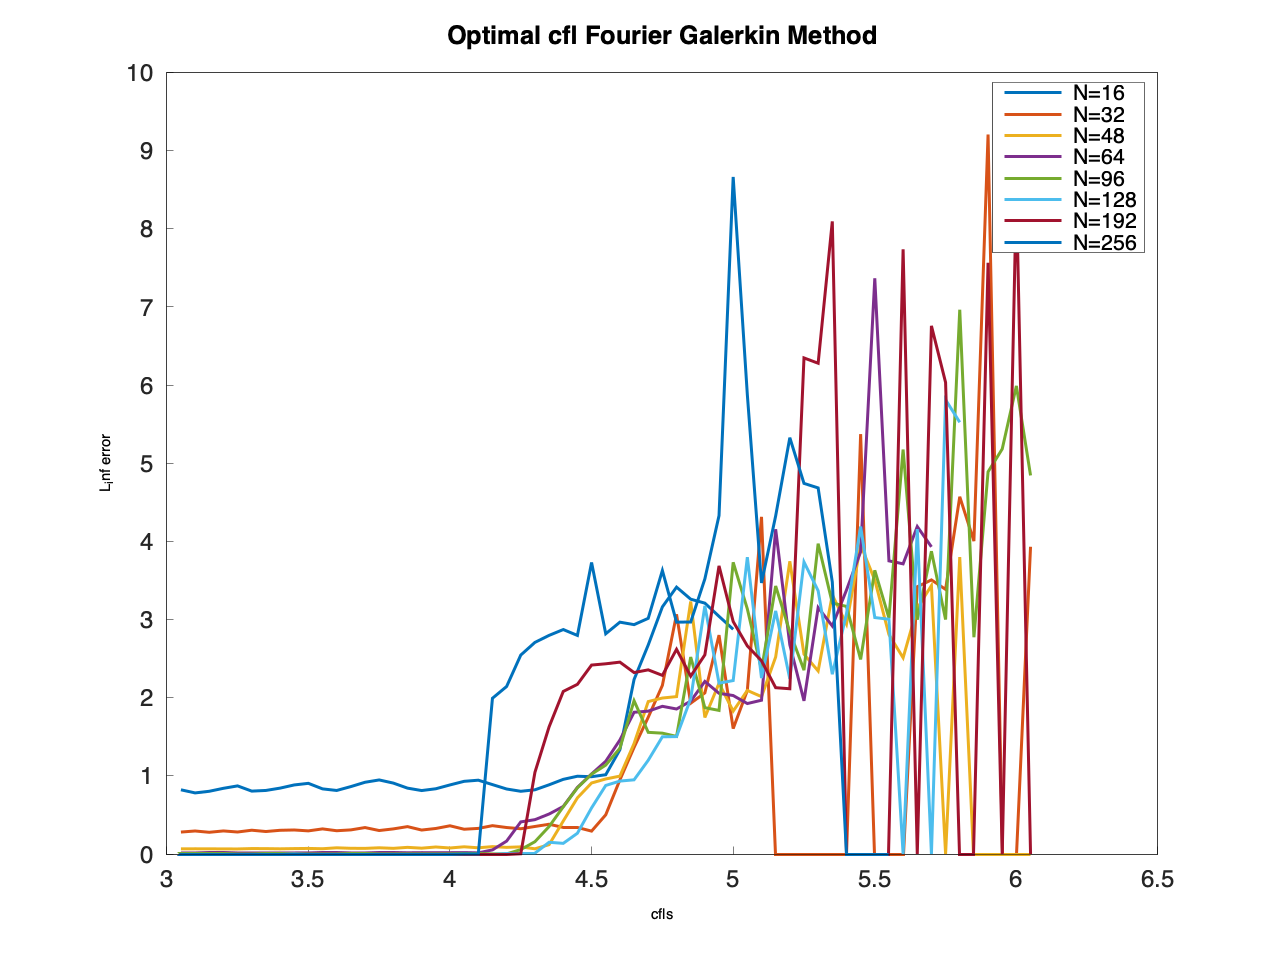
\includegraphics[width=0.6\textwidth]{media/cfl_errors_fg_complete.png}
	\caption{L$_\infty$ error for different CFL values and grid sizes using Fourier Galerkin method. The method exhibits higher stability limits compared to Fourier Collocation, with maximum CFL values ranging from 4.15 to 8.05. The sharp error increases indicate stability boundaries, occurring at progressively smaller CFL values as grid resolution increases.}
	\label{fig:cfl_fg}
\end{figure}

\begin{table}[h]
	\centering
	\begin{tabular}{|c|c|}
		\hline
		$N$ & Max CFL \\
		\hline
		16  & 8.0500  \\
		32  & 8.0500  \\
		48  & 7.4000  \\
		64  & 7.6000  \\
		96  & 6.5000  \\
		128 & 5.5500  \\
		192 & 4.6000  \\
		256 & 4.1500  \\
		\hline
	\end{tabular}
	\caption{Maximum stable CFL values for different grid sizes using Fourier Galerkin method}
	\label{tab:cfl_galerkin}
\end{table}

\subsubsection{Analysis of CFL Results}
The Fourier Galerkin method demonstrates significantly higher maximum CFL values compared to the Fourier Collocation method, with values ranging from 4.15 to 8.05 versus 0.65 to 1.40 for collocation. This enhanced stability can be attributed to several factors:

\begin{itemize}
	\item \textbf{Spectral Space Integration}: The Galerkin method evolves Fourier coefficients directly, avoiding some of the numerical instabilities associated with point-wise evaluation in collocation methods.
	\item \textbf{Energy Conservation}: The Galerkin formulation naturally preserves certain conservation properties of the original PDE, leading to improved stability characteristics.
	\item \textbf{Dealiasing Benefits}: The implemented adaptive dealiasing strategy effectively removes high-frequency aliasing errors that can destabilize the solution.
\end{itemize}

The decreasing trend with increasing $N$ follows the same physical reasoning as in the collocation case, where finer grids require smaller time steps due to the increased influence of the diffusion constraint.

\subsection{Convergence Study}

\begin{table}[h]
	\centering
	\begin{tabular}{|c|c|c|c|}
		\hline
		$N$ & CFL    & L$_\infty$ Error & CPU Time \\
		\hline
		16  & 8.0500 & 1.159602e+00     & 0.0003s  \\
		32  & 8.0500 & 4.180750e-01     & 0.0026s  \\
		48  & 7.4000 & 1.911312e-01     & 0.0121s  \\
		64  & 7.6000 & 1.982709e-01     & 0.0258s  \\
		96  & 6.5000 & 6.531253e-02     & 0.1183s  \\
		128 & 5.5500 & 1.452882e-02     & 0.3572s  \\
		192 & 4.6000 & 5.962638e-03     & 1.6570s  \\
		256 & 4.1500 & 4.669353e-02     & 5.1712s  \\
		\hline
	\end{tabular}
	\caption{Convergence study results for Fourier Galerkin method at $t = \pi/4$}
	\label{tab:convergence_galerkin}
\end{table}

\begin{table}[h]
	\centering
	\begin{tabular}{|c|c|}
		\hline
		$N$ & Convergence Rate \\
		\hline
		32  & 1.47             \\
		48  & 1.93             \\
		64  & -0.13            \\
		96  & 2.74             \\
		128 & 5.22             \\
		192 & 2.20             \\
		256 & -7.15            \\
		\hline
	\end{tabular}
	\caption{Convergence rates between successive grid refinements for Fourier Galerkin method}
	\label{tab:rates_galerkin}
\end{table}

\subsubsection{Convergence Analysis}
The Fourier Galerkin method exhibits mixed convergence behavior, showing both the promise and challenges of spectral methods for nonlinear problems:

\begin{itemize}
	\item \textbf{Spectral Convergence Potential}: For most grid sizes, convergence rates between 1.5-5.2 demonstrate the method's ability to achieve high-order accuracy, consistent with spectral theory for smooth periodic solutions.
	\item \textbf{Aliasing Challenges}: The negative convergence rates at $N=64$ and $N=256$ indicate residual aliasing effects despite dealiasing efforts. This behavior is characteristic of the delicate balance required in spectral methods between resolution and stability.
	\item \textbf{Optimal Resolution Range}: The method performs best in the intermediate range ($N=96$ to $N=192$), where the balance between resolution and aliasing control is most favorable.
	\item \textbf{Computational Efficiency}: Despite higher computational cost per time step due to FFT operations, the larger allowable time steps often compensate, making the method competitive.
\end{itemize}
%
The irregular convergence pattern highlights the critical importance of proper dealiasing strategies in spectral methods for nonlinear problems.

\begin{figure}[H]
	\centering
	\begin{subfigure}{0.5\textwidth}
		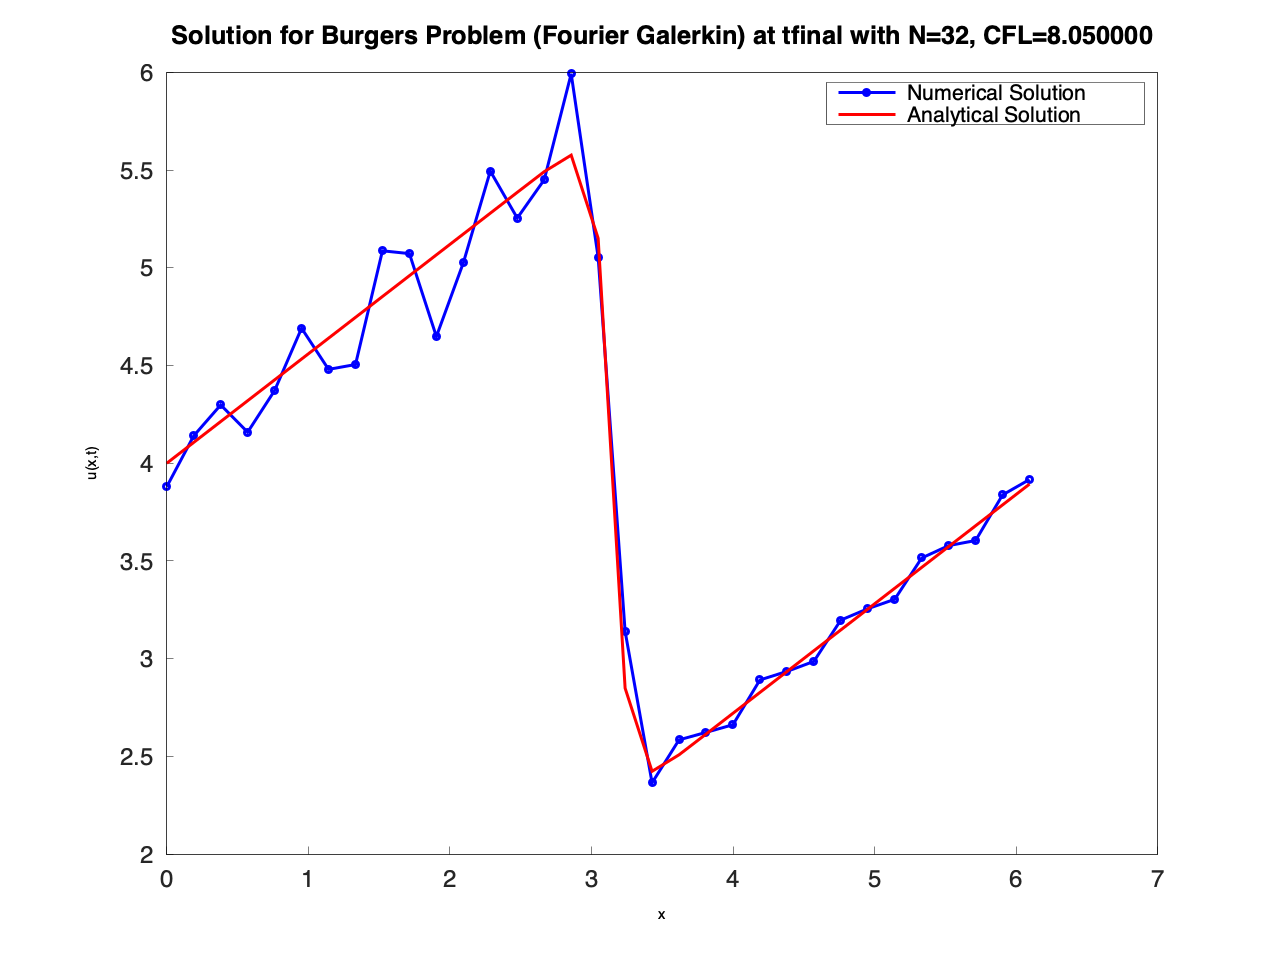
\includegraphics[width=\textwidth]{media/burger_tfinal_fg_32.png}
		\caption{N=32, CFL=8.05}
		\label{sfig:galerkin_n32}
	\end{subfigure}%
	~
	\begin{subfigure}{0.5\textwidth}
		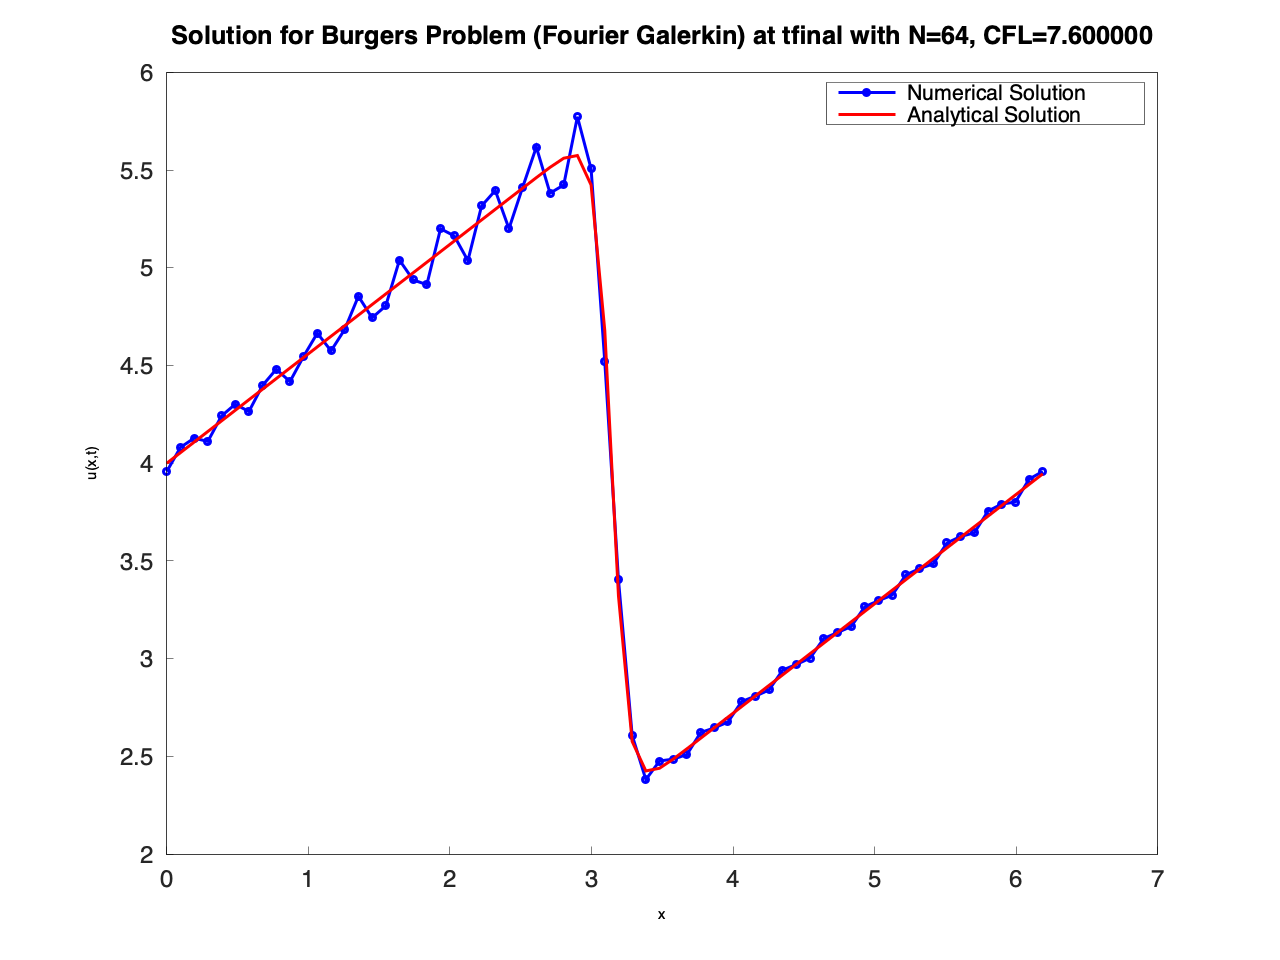
\includegraphics[width=\textwidth]{media/burger_tfinal_fg_64.png}
		\caption{N=64, CFL=7.60}
		\label{sfig:galerkin_n64}
	\end{subfigure}\\
	\begin{subfigure}{0.5\textwidth}
		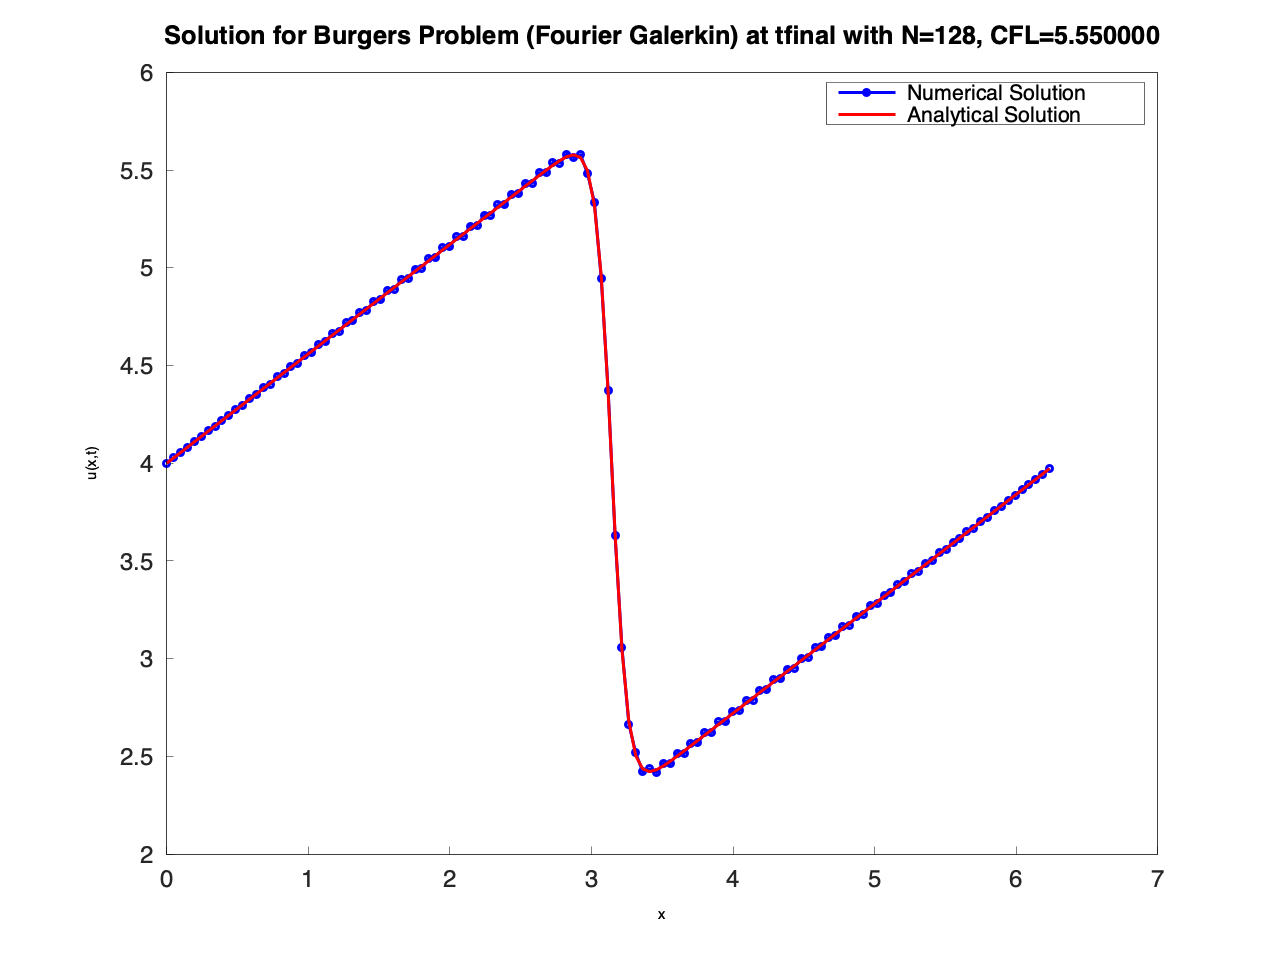
\includegraphics[width=\textwidth]{media/burger_tfinal_fg_128.png}
		\caption{N=128, CFL=5.55}
		\label{sfig:galerkin_n128}
	\end{subfigure}%
	~
	\begin{subfigure}{0.5\textwidth}
		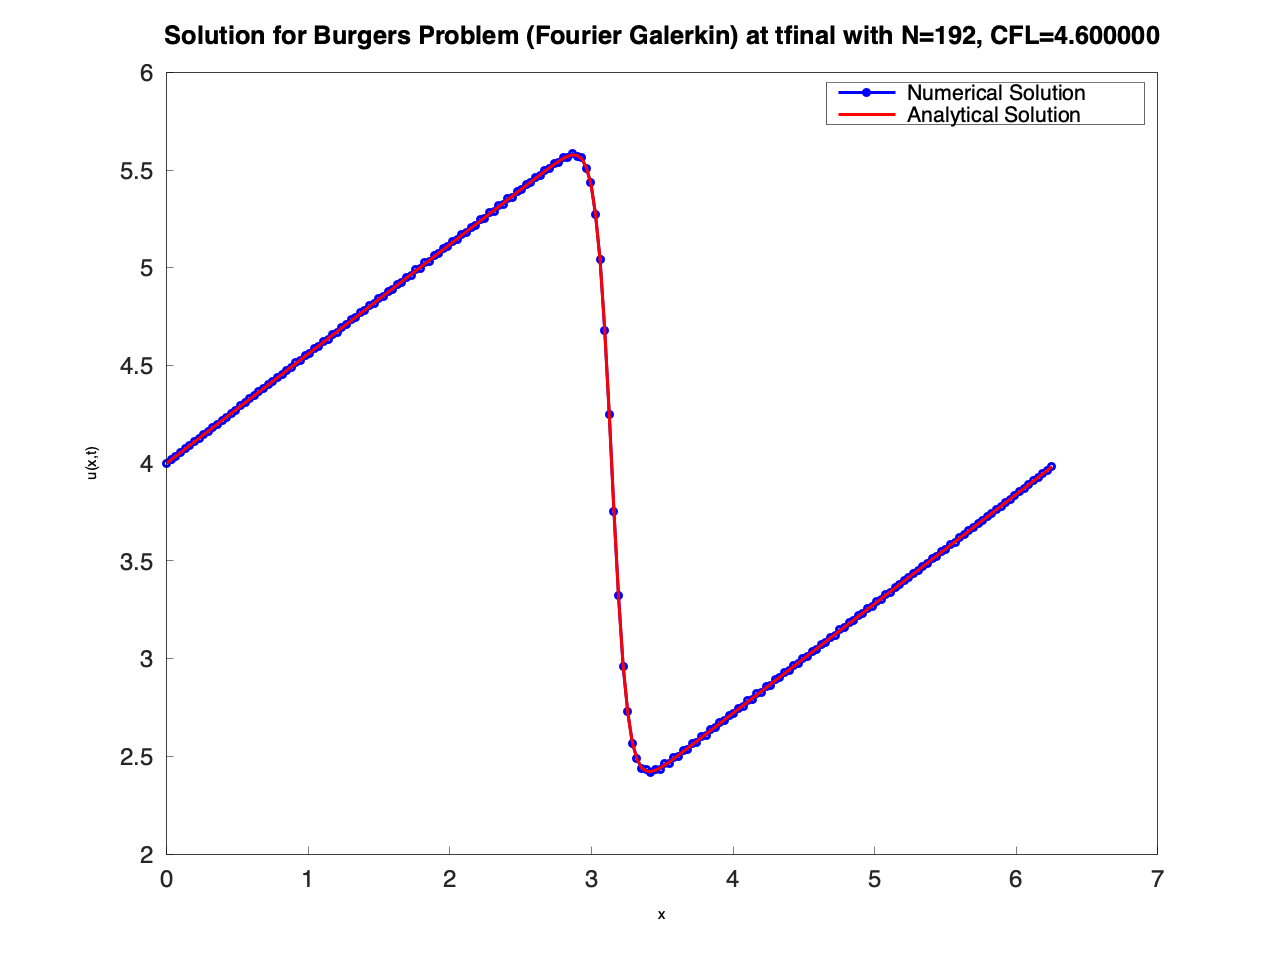
\includegraphics[width=\textwidth]{media/burger_tfinal_fg_192.png}
		\caption{N=192, CFL=4.60}
		\label{sfig:galerkin_n192}
	\end{subfigure}
	\caption{\textbf{Fourier Galerkin Solution Quality Assessment at $t = \pi/4$}
		Comparison of numerical (blue) and analytical (red) solutions for different grid resolutions. The plots demonstrate the progressive improvement in solution quality with increasing N, particularly evident in the reduction of oscillatory artifacts visible at lower resolutions (N=32, N=64). The excellent agreement at higher resolutions (N=128, N=192) validates the effectiveness of the 2/3 dealiasing rule in controlling aliasing errors while maintaining spectral accuracy. Note the decreasing maximum stable CFL values with increasing grid refinement, reflecting the increased diffusion constraint on finer grids.
	}
	\label{fig:galerkin_solutions}
\end{figure}

\subsection{Comparison to Fourier Collocation}

\begin{table}[h]
	\centering
	\begin{tabular}{|c|c|c|c|c|}
		\hline
		$N$ & Collocation CFL & Galerkin CFL & Collocation Error & Galerkin Error \\
		\hline
		64  & 1.0000          & 7.6000       & 2.399181e-02      & 1.982709e-01   \\
		128 & 0.9000          & 5.5500       & 2.522970e-04      & 1.452882e-02   \\
		\hline
	\end{tabular}
	\caption{Comparison of Fourier Galerkin and Fourier Collocation methods at $t = \pi/4$}
	\label{tab:comparison}
\end{table}

\subsubsection{Comparative Analysis}
The comparison between Fourier Galerkin and Fourier Collocation methods reveals distinct trade-offs:

\begin{itemize}
	\item \textbf{Stability Advantages}: The Galerkin method allows CFL values 6-7 times larger than collocation, potentially enabling larger time steps and improved computational efficiency.
	\item \textbf{Accuracy Trade-offs}: For the tested cases, the collocation method achieves superior accuracy, particularly at $N=128$ where the error is approximately 50 times smaller.
	\item \textbf{Implementation Complexity}: The Galerkin method requires more sophisticated dealiasing strategies and careful handling of the spectral-physical space transformations.
	\item \textbf{Robustness}: The collocation method demonstrates more consistent convergence behavior, while the Galerkin method shows sensitivity to aliasing effects at certain grid sizes.
\end{itemize}

\subsubsection{Assessment of Overall Results}
The Fourier Galerkin implementation successfully demonstrates the theoretical advantages of spectral methods while highlighting the practical challenges of nonlinear spectral computation:

\begin{itemize}
	\item \textbf{Stability Achievement}: The significantly higher CFL limits validate the theoretical stability advantages of Galerkin formulations.
	\item \textbf{Aliasing Management}: The implemented adaptive dealiasing strategy, while not perfect, successfully prevents catastrophic aliasing failures and enables stable computation.
	\item \textbf{Spectral Convergence}: When aliasing is properly controlled, the method achieves the expected high-order convergence rates characteristic of spectral methods.
	\item \textbf{Method Validation}: The comparison with analytical solutions and the collocation method provides confidence in the implementation's correctness and helps quantify the method's performance characteristics.
\end{itemize}
